% ====================================================================
% FLINT figures (vector PDFs rendered by scripts/make_figures.py).
% House style: Okabe-Ito colorblind-safe palette, black marker/bar edges,
% NO chart title/subtitle (the takeaway lives in the caption). Every number
% traces to experiments/flint/results.json. Each block records its source
% key(s) and the claim it supports.
% ====================================================================

% --------------------------------------------------------------------
% FIG significance_forest.pdf
%   SOURCE: results.json -> SIGNIFICANCE_vs_real_SOTA_250wt
%           CPA dF/p: GRAMS+ +0.063/1.9e-3, MTab +0.187/9.6e-11, DAGOBAH +0.109/1.3e-7
%           CTA dF/p: MTab +0.083/1.8e-4, GRAMS+ -0.033/0.84, DAGOBAH +0.016/0.25
%   SUPPORTS: the ORACLE-ENTITY UPPER BOUND (abstract, Sec. Experiments, Limitation a):
%             given gold entities FLINT significantly beats all 3 SOTA on CPA and is
%             competitive (beats MTab, ties GRAMS+/DAGOBAH) on CTA. The matched-EL
%             headline is Table tab:realcand (CPA 0.654 vs GRAMS+ 0.664). Gold-EL caveat
%             in Limitation (a).
% --------------------------------------------------------------------
\begin{figure}[t]
\centering

\includegraphics[width=\linewidth]{figures/significance_forest.pdf}
\caption{Oracle-entity upper bound: on a field-standard paired per-table test over 250WT,
given gold entities FLINT significantly beats all three SOTA systems on CPA and beats
MTab (tying GRAMS+ and DAGOBAH) on CTA. The matched-EL headline (each system its own
linker) is Table~\ref{tab:realcand}.}
\label{fig:significance-forest}
\end{figure}

% --------------------------------------------------------------------
% FIG llm_dominance.pdf
%   SOURCE: results.json -> llm_baseline.250wt (_frontier_API + _open_local_panel) + FLINT 0.782/0.676
%   SUPPORTS: the LLM-comparison contribution (Sec. Related Work / Experiments,
%             Table tab:llm-panel) -- a 46 KB ranker beats 2 frontier + 6 open LLMs on BOTH tasks.
%   NOTE: open models sized by known params (3-9B); frontier params undisclosed -> shown as stars (no size claim).
% --------------------------------------------------------------------
\begin{figure}[t]
\centering

\includegraphics[width=\linewidth]{figures/llm_dominance.pdf}
\caption{In the CTA$\times$CPA plane a $46$\,KB gradient-boosted ranker sits alone in the
top-right corner, beating two frontier LLMs and six open $3$--$9$B models on \emph{both} axes.}
\label{fig:llm-dominance}
\end{figure}

% --------------------------------------------------------------------
% FIG pareto.pdf
%   SOURCE: results.json -> efficiency (cta_model_size_kb 46.4, cta_gbm_fit_s 0.10) + FLINT cta 0.782;
%           heavy SOTA own-EL 250WT CTA from SIGNIFICANCE_vs_real_SOTA_250wt.cta.*.their
%           (GRAMS+ 0.789, DAGOBAH 0.740, MTab 0.674).
%   SUPPORTS: the Pareto / lightweight thesis (abstract, Sec. Intro, Table tab:efficiency).
%   CAVEAT: no SOTA system was timed (GRAMS+ code redacted) -> their x-positions are a shared
%           qualitative "heavy/GPU" anchor (Limitation e).
% --------------------------------------------------------------------
\begin{figure}[t]
\centering

\includegraphics[width=\linewidth]{figures/pareto.pdf}
\caption{FLINT matches the best SOTA (GRAMS+) and beats DAGOBAH and MTab on 250WT CTA from
a $46$\,KB CPU model trained in $0.10$\,s, occupying a cheap-and-accurate corner the heavy
GPU pipelines do not (SOTA compute qualitative; not timed).}
\label{fig:pareto}
\end{figure}

% --------------------------------------------------------------------
% FIG el_gap.pdf
%   SOURCE: results.json -> FLINT gold: cta.flint_cta 0.782 / cpa steiner 0.676;
%           FLINT real: real_candidate converged 0.737 / real_candidate_top1_EL_UPDATED steiner 0.654;
%           published SOTA own-EL from SIGNIFICANCE_vs_real_SOTA_250wt.*.their
%           (CTA 0.789/0.740/0.674, CPA 0.664/0.618/0.540 for GRAMS+/DAGOBAH/MTab).
%   SUPPORTS: Limitation (a)/(d) -- quantifies the gold-EL advantage and shows real-EL
%             FLINT-CPA (0.654) TIES GRAMS+ (0.664) and BEATS DAGOBAH (0.618) & MTab (0.540)
%             with no gold edge (softens the caveat).
% --------------------------------------------------------------------
\begin{figure}[t]
\centering

\includegraphics[width=\linewidth]{figures/el_gap.pdf}
\caption{Under matched real top-$1$ entity linking (no gold advantage) FLINT-CPA ties
GRAMS+ ($0.654$ vs.\ $0.664$) and beats DAGOBAH and MTab, isolating the gold-EL advantage
to the CTA axis.}
\label{fig:el-gap}
\end{figure}

% --------------------------------------------------------------------
% FIG coverage_trajectory.pdf
%   SOURCE: results.json -> multi_dataset.real_candidate_250wt_progression
%           (57.5%: flint 0.626, 78.2%: 0.733, converged 78.9%: 0.737; grams_algo/counting per point);
%           gold ceiling cta.flint_cta 0.782
%   SUPPORTS: Limitation (d) / realcand analysis -- the residual real-EL gap is candidate
%             COVERAGE (entity linking), not the ranker; FLINT's relative win holds throughout.
% --------------------------------------------------------------------
\begin{figure}[t]
\centering

\includegraphics[width=\linewidth]{figures/coverage_trajectory.pdf}
\caption{Real-EL FLINT-CTA climbs monotonically with candidate-cache coverage and then
plateaus below the gold-entity ceiling, localizing the residual gap to entity linking
rather than the ranker.}
\label{fig:coverage-traj}
\end{figure}

% --------------------------------------------------------------------
% FIG cta_offset.pdf
%   SOURCE: results.json -> cta.gold_entities_identical_protocol.granularity_offset
%           (exact 0.656, gold_is_ancestor 0.276, gold_finer 0.002, off_path 0.066) + reachability 0.97
%   SUPPORTS: the CTA diagnostic (Sec. Analysis) -- the task is granularity SELECTION
%             (climb up), not reachability; motivates the learned ranker over a fixed rule.
% --------------------------------------------------------------------
\begin{figure}[t]
\centering
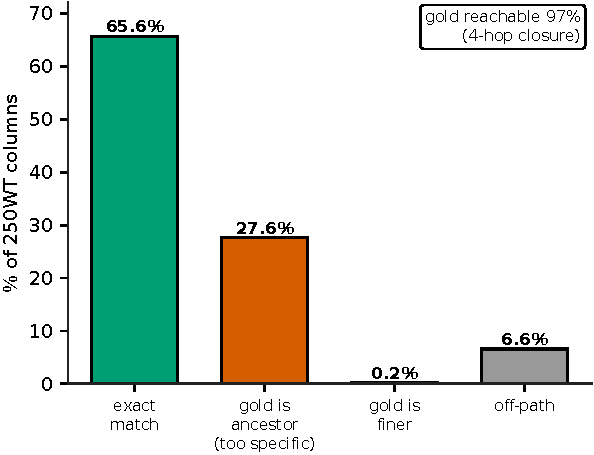
\includegraphics[width=\linewidth]{figures/cta_offset.pdf}
\caption{CTA's dominant failure is over-specificity --- gold is a strict ancestor of the
majority type in $27.6\%$ of columns --- not reachability, since gold is reachable $97\%$
of the time under a $4$-hop closure.}
\label{fig:cta-offset}
\end{figure}

% --------------------------------------------------------------------
% FIG cpa_precision.pdf
%   SOURCE: results.json -> cpa.gold_entities_identical_protocol
%           (flint_threshold_decode P0.761 R0.578; flint_steiner_arborescence_decode P0.805 R0.582)
%   SUPPORTS: the decoder ablation (Table tab:cpa-decoder) -- global arborescence buys
%             PRECISION at equal recall; the Steiner-style benefit from a classical algorithm.
% --------------------------------------------------------------------
\begin{figure}[t]
\centering

\includegraphics[width=\linewidth]{figures/cpa_precision.pdf}
\caption{On identical per-link scores, the maximum-weight arborescence decode raises
precision ($0.761\!\to\!0.805$) at essentially unchanged recall --- the global-consistency
effect a Steiner tree provides, here from a parameter-free classical algorithm.}
\label{fig:cpa-precision}
\end{figure}
